\section{SoundnessBench: Benchmark Reconstruction}

\begin{figure}[t]
    \centering
    % PLACEHOLDER: Figure 1 — full pipeline (5-step diagram)
    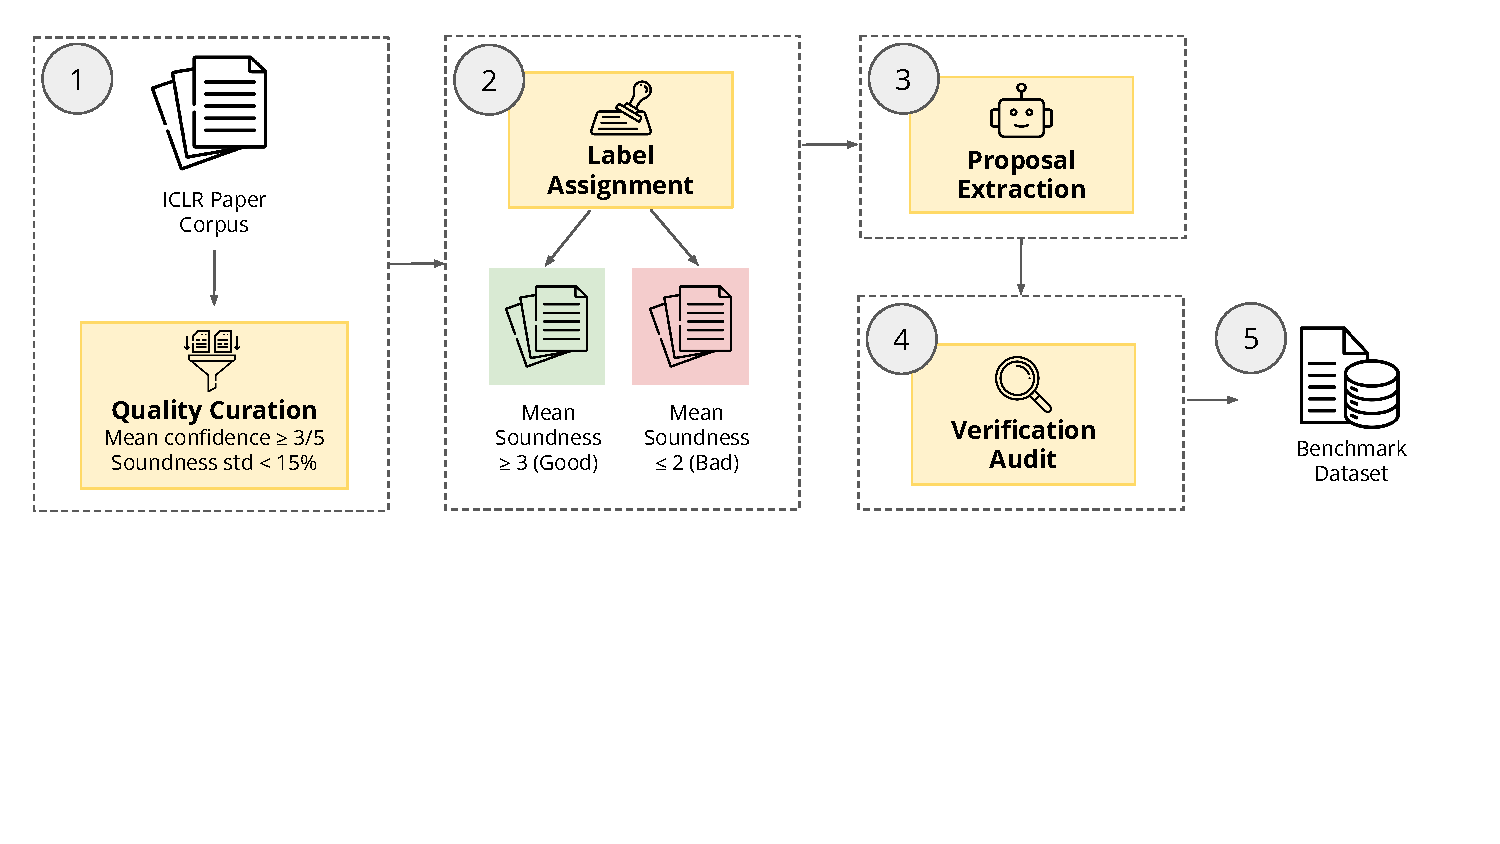
\includegraphics[trim={0 5.5cm 1cm 0},clip,width=\linewidth]{figures/pipeline.pdf}
    \caption{\textbf{SoundnessBench pipeline:} (1) collect ICLR papers with reviewer metadata and filter for high reviewer agreement; (2) derive high/low-soundness labels; (3) extract a near-verbatim research proposal without revealing experimental results; (4) audit extraction fidelity with retrieve-then-verify atomic claims; and (5) assemble the final benchmark.}
    \label{fig:pipeline}
\end{figure}


\begin{figure}[t]
    \centering
    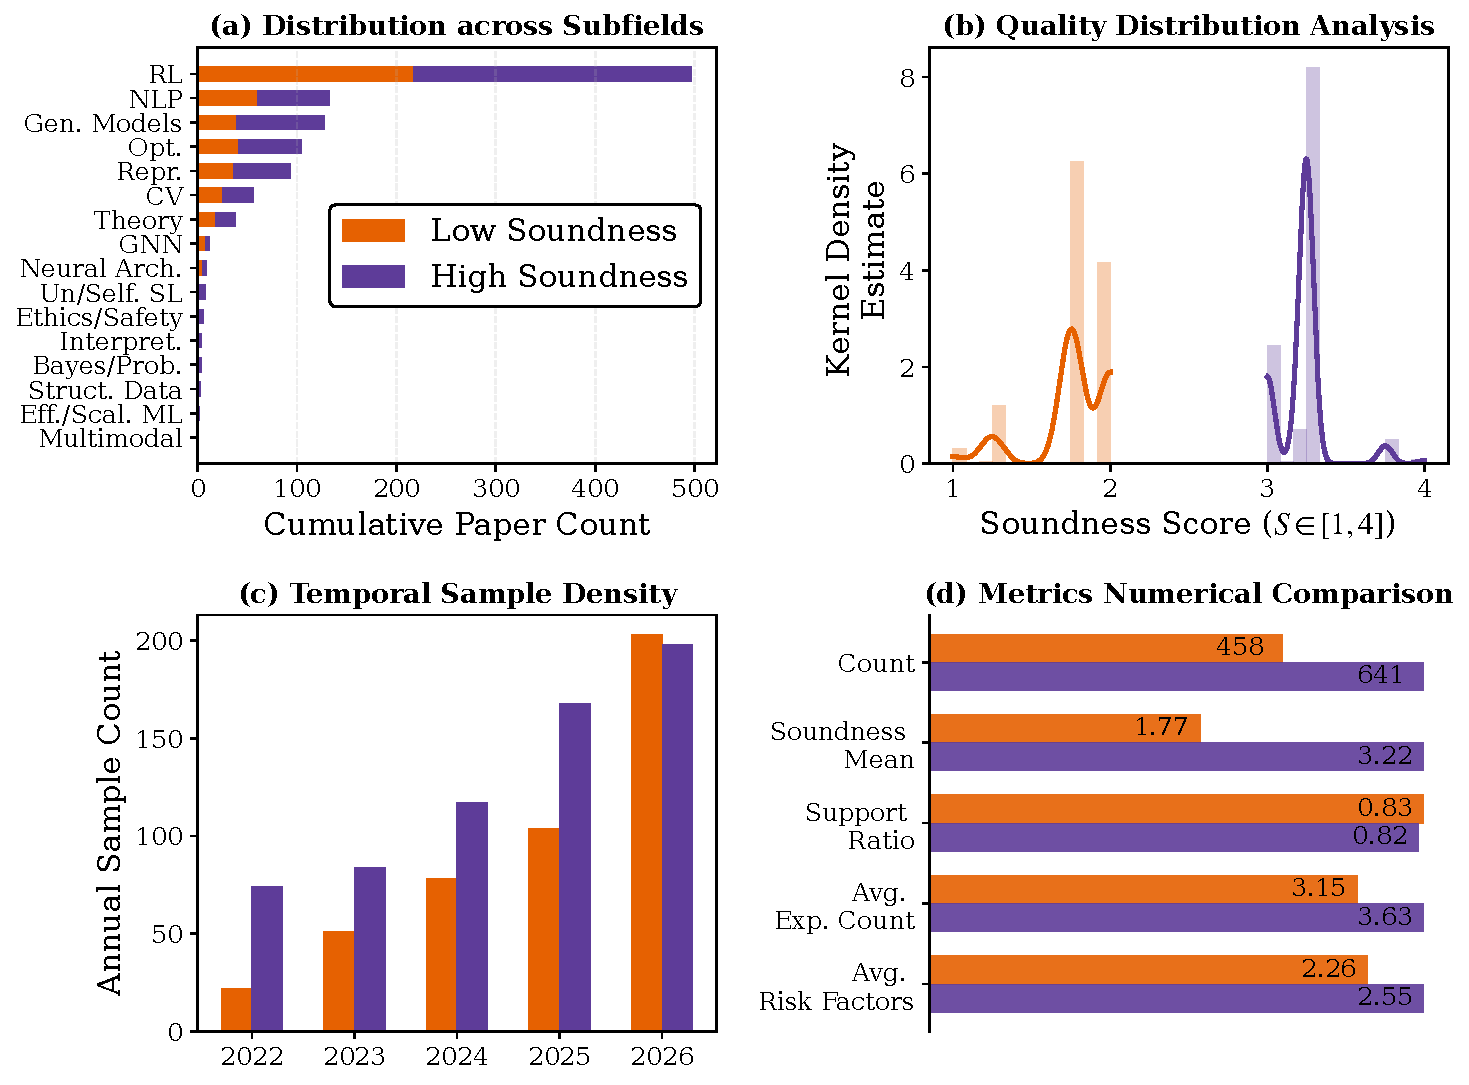
\includegraphics[width=0.95\linewidth]{figures/dataset_stats.pdf}
    \caption{\textbf{SoundnessBench dataset statistics.} The benchmark contains 1,099 proposals, including 458 low-soundness and 641 high-soundness instances. \textbf{(a)} The subfield distribution across papers reflects the ICLR corpus composition. \textbf{(b)} Soundness score density shows separation between low-soundness ($S \leq 2$, mean $= 1.77$) and high-soundness ($S \geq 3$, mean $= 3.22$) groups, supporting the chosen label boundary. \textbf{(c)} Temporal coverage spans ICLR 2022--2026. \textbf{(d)} Low- and high-soundness pair-count statistics in SoundnessBench.}
    \label{fig:stats}
\end{figure}

\textbf{Overview and Motivation.}
In human research, the first gate happens before implementation: researchers and advisors ask whether a hypothesis is well-posed and whether the planned experiment can truly validate or falsify the claim. This early judgment decides which ideas deserve months of engineering effort and compute.

SoundnessBench targets this first-gate setting for LLM agents. Most existing LLM benchmarks evaluate downstream skills (writing, coding, or reviewing completed papers), with limited direct testing of whether an agent can reject weak designs before execution. SoundnessBench addresses this gap by isolating pre-execution rigor assessment, grounding labels in peer-review outcomes, and auditing extraction faithfulness so each instance is traceable to source evidence. In short, it probes how well current LLM-based agents can make early-stage soundness judgments from proposal text alone.

% \paragraph{Challenges and Design Choices.} Constructing a proposal-only soundness benchmark from real submissions required us to address three challenges up front. First, \textit{label reliability}: reviewer judgments can be noisy and mixed, so we use ICLR reviewer soundness scores as a proxy, keep only high-agreement reviews, and remove ambiguous middle-score cases. Second, \textit{information leakage}: completed papers contain results that can shortcut true first-gate assessment, so we exclude experimental outcomes and keep only proposal components. Third, \textit{extraction fidelity}: proposal extraction can introduce drift, so we preserve near-verbatim wording and add a retrieval-backed atomic-claim verification audit.
\paragraph{\fh{Challenges and Design Choices.}} \fh{Constructing a proposal-only soundness benchmark from real submissions required us to address four challenges up front. First, \textit{label reliability}: reviewer judgments can be noisy and mixed, so we use ICLR reviewer soundness sub-scores as a proxy for methodological validity, keep only high-agreement reviews, and remove ambiguous middle-score cases. Second, \textit{label scope}: reviewers saw full papers, while our models see results-masked proposals; therefore SoundnessBench measures recoverable proposal-stage soundness rather than exact prediction of full-paper review outcomes. Third, \textit{information leakage}: completed papers contain results and acceptance cues that can shortcut true first-gate assessment, so we exclude experimental outcomes and keep only proposal components. Fourth, \textit{extraction fidelity}: proposal extraction can introduce drift, so we preserve near-verbatim wording, require source-grounded extraction, and add retrieval-backed atomic-claim verification.}

We chose these design decisions to maximize reliability, task faithfulness, and traceability at the same time. Compared with prior benchmarks that emphasize downstream tasks or rely primarily on post-hoc annotation, SoundnessBench explicitly combines peer-review-grounded labels, proposal-only inputs, and evidence-audited extraction, which enables a cleaner test of pre-execution scientific judgment.

\textbf{Benchmark Reconstruction.}
We build SoundnessBench in five steps, shown in Fig.~\ref{fig:pipeline}.

\begin{itemize}[leftmargin=*,itemsep=0.1in, topsep=0in, parsep=0in]
    \item \textbf{Step 1: Data Collection.} We collect papers from the ICLR corpus, covering major ML areas such as RL, generative modeling, NLP, optimization, and computer vision (16 subfields in total). We start from 2022 because earlier releases do not consistently provide reviewer soundness (or closely related) scores needed for filtering and label derivation. This multi-year, multi-subfield pool helps reduce narrow-domain bias. From the collected papers, we remove desk-rejected papers, since desk rejections may reflect factors other than scientific soundness. Then, to reduce label noise, we retain only papers with strong reviewer agreement: mean reviewer confidence of at least 3 and a standard deviation of normalized soundness scores below 0.15.
    \item \textbf{Step 2: Label Assignment.} \fh{We assign labels from reviewer \emph{soundness} sub-scores rather than overall ratings, acceptance decisions, or novelty/presentation scores. Pairs with mean soundness scores $\geq 3$ are labeled \textit{high} soundness, whereas pairs with mean scores $\leq 2$ are labeled \textit{low} soundness. Ambiguous middle-score cases are excluded to improve class separation. These labels are expert-derived proxies for recoverable proposal-stage methodological validity, not claims of absolute or post-execution research quality.}
    \item \textbf{Step 3: Proposal Extraction.} \fh{From the papers filtered in Step 2, we extract a research proposal including the abstract, related work, risk factors, hypothesis, and experiment design directly from source PDFs, while excluding experimental results, direct outcome claims, and acceptance cues. The proposal format follows The AI Scientist-v2~\citep{yamada2025aiscientistv2}. We preserve near-verbatim wording to reduce paraphrase drift and keep inputs aligned with the original submissions. We use a strong long-context LLM (Gemini 2.5 Pro) with a task-specific prompt that requires source-grounded spans and forbids unsupported inference (Supplementary Sec.~\ref{sec:supp:prompt-extract}). Example extractions are provided in Supplementary Sec.~\ref{sec:supp:proposal-examples}.}
    \item \textbf{Step 4: Verification Audit.} To ensure the extracted proposals faithfully match source PDFs and to minimize extraction errors from Step 3, we add a verification audit. The detailed process is presented in Alg.~\ref{alg:verification}. We check extraction faithfulness with a retrieval-backed atomic-claim score. Following prior work on atomic factuality and evidence-grounded verification~\citep{min-etal-2023-factscore,thorne2018fever}, we decompose each extracted hypothesis--experiment pair into atomic claims, retrieve supporting passages, and verify each claim against the source paper (Supplementary Sec.~\ref{sec:supp:prompt-decompose}, Sec.~\ref{sec:supp:prompt-verify}, and Sec.~\ref{sec:supp:atomic-example}). We set threshold $\tau=0.7$, chunk size $\ell=3000$, chunk overlap $o=200$, and retrieval depth $k=3$. In our current pool, 66.93\% of candidates pass this filter, yielding a benchmark with auditable hypothesis--experiment designs. The mean support ratio is shown in Fig.~\ref{fig:stats}.

    \item \textbf{Step 5: Final Benchmark Dataset.} The final benchmark contains 1,099 research proposals, including 458 low-soundness and 641 high-soundness instances. Detailed benchmark statistics are presented in Fig.~\ref{fig:stats}.
\end{itemize}

\begin{algorithm}[ht]
\caption{Verification Audit}
\label{alg:verification}
\begin{algorithmic}[1]
\Require Source PDF $\mathcal{P}$, extracted pair $\hat{p} = (h, e)$, 
         threshold $\tau$, chunk size $\ell$, chunk overlap $o$, retrieval depth $k$
\Ensure Fidelity score $\rho \in [0, 1]$, and binary pass/fail decision

\State $\mathcal{T} \leftarrow \textsc{ExtractText}(\mathcal{P})$
\State $\mathcal{C} \leftarrow \textsc{Chunk}(\mathcal{T},\ \ell,\ o)$
\State $\mathcal{A} \leftarrow \textsc{DecomposeAtomicClaims}(\hat{p})$
\State $\text{supported} \leftarrow 0$

\For{each claim $c \in \mathcal{A}$}
    \State $\mathcal{E} \leftarrow \textsc{BM25}(c,\ \mathcal{C},\ \text{top-}k=k)$
    \State $v \leftarrow \textsc{LLMVerify}(c,\ \mathcal{E},\ \text{evidence\_only}=\texttt{True})$
    \If{$v = \texttt{YES}$}
        \State $\text{supported} \leftarrow \text{supported} + 1$
    \EndIf
\EndFor

\State $\rho \leftarrow \text{supported}\ /\ |\mathcal{A}|$
\State \Return $(\rho,\ \rho \geq \tau)$

\end{algorithmic}
\end{algorithm}


% Reliability is supported by three controls: reviewer-agreement filtering for cleaner labels, evidence-grounded verification for extraction faithfulness, and transparent class-distribution reporting for robust evaluation. Together, these controls aim to reduce annotation noise and improve comparability across models.

